\documentclass[11pt,letterpaper]{article}
\usepackage[margin=1.0in]{geometry}
\usepackage[utf8]{inputenc}
\usepackage{cite}
\usepackage{amsmath}
\usepackage{amsfonts}
\usepackage{amssymb}
\usepackage{makeidx}
\usepackage{graphicx}
\usepackage{hyperref}
\setlength\parindent{0pt}

\author{STUDENT NAME}
\title{HW: Fourier series of a triangular signal}

\begin{document}

\maketitle

\textbf{Introduction}

If a signal is given on an interval $[0, 2 \pi]$, the Fourier series can be written as:

\begin{equation}\label{HW_FourierSeries1}
f(t) = c_0 + \sum\limits_{n=1}^{\infty} a_n \cos nt + b_n \sin nt 
\end{equation}

with coefficients:

\begin{align}\label{HW_FourierSeries2}
 & c_0=\frac{1}{2\pi }\int\limits_{0}^{2\pi }{f\left( t \right)dt} \\ 
 & a_n=\frac{1}{\pi }\int\limits_{0}^{2\pi }{f\left( t \right)\cos ntdt} \\ 
 & b_n=\frac{1}{\pi }\int\limits_{0}^{2\pi }{f\left( t \right)\sin ntdt}
\end{align}

\textbf{Worked example 1}

Figure \ref{fig:HW_FourierSeries1} shows a square wave given on the interval $[0, 2 \pi]$. To calculate the Fourier coefficients, we need to evaluate the integrals above, but you need to be smart about it. Firstly, the coefficient $c_0$ represents the mean of the signal, and just by looking at the signal you can tell $c_0$ will be zero. Secondly, as you know, if a signal is even, then only coefficients of cosine will have a value, because the cosine itself is an even function. Vice versa for an odd function where only the sine coefficients will have a value. By the way, some signals are both odd and even, then both sine and cosine coefficients will have a value. Since our function is obviously odd (it is symmetric in the origin) only the sine coefficients will have a value therefore $a_n = 0$. The values of the sine coefficients can be calculated by evaluating the integral:

\begin{figure}
\centering
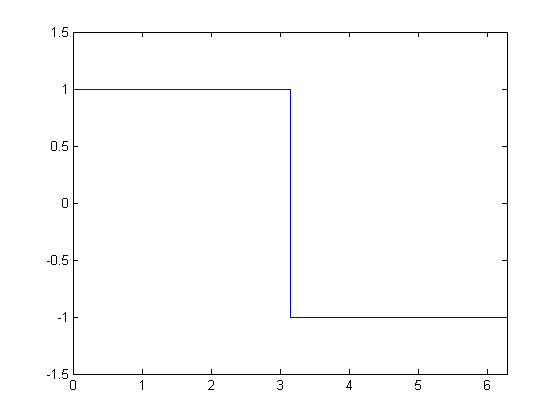
\includegraphics[width=0.7\linewidth]{HW_FourierSeries1}
\caption{Square wave signal on the interval $[0, 2 \pi]$.}
\label{fig:HW_FourierSeries1}
\end{figure}

For the part of the signal that runs from $0$ to $\pi$ we get:

\begin{equation}\label{HW_FourierSeries4}
b_n = \dfrac{1}{\pi} \int \limits_{0}^{\pi} sin(nt) dt =  \dfrac{-1}{n\pi} \left| cos(nt) \right|_0^\pi = \dfrac{-1}{n\pi}\left| cos(n\pi) -cos(0) \right|
\end{equation}
The values of the $b_n$ coefficients for the interval $0, \pi$ are now $0$ for $n$ = even, and $\dfrac{2}{n \pi}$ for $n$ = odd.\\

For the part of the signal that runs from $\pi$ to $2 \pi$ we get:

\begin{equation}\label{HW_FourierSeries5}
b_n = \dfrac{1}{\pi} \int \limits_{\pi}^{2 \pi} -sin(nt) dt =  \dfrac{1}{n\pi} \left| cos(nt) \right|_\pi ^{2\pi} = \dfrac{1}{n\pi}\left| cos(2n\pi) -cos(n\pi) \right|
\end{equation}

The values of the $b_n$ coefficients for the interval $\pi, 2 \pi$ are now $0$ for $n$ = even, and $\dfrac{2}{n \pi}$ for $n$ = odd. 

The sum of $b_n$ coefficients for the interval $0, 2 \pi$ are now $0$ for $n$ = even and $\dfrac{4}{n \pi}$ for $n$ = odd. The spectrum where the coefficient values are plotted against the frequency (coefficient number $n$) is shown in Figure \ref{fig:HW_FourierSeries2}. The first two coefficients are $\dfrac{4}{\pi} = 1.2732 (n=1)$, $\dfrac{4}{3 \pi} = 0.4244 (n=3)$, verify this in Figure \ref{fig:HW_FourierSeries2}.\\

\begin{figure}
\centering
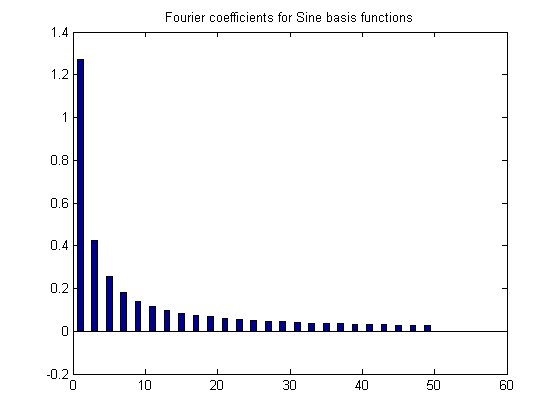
\includegraphics[width=0.7\linewidth]{HW_FourierSeries2}
\caption{Fourier coefficients of a square wave signal on the interval $[0, 2 \pi]$.}
\label{fig:HW_FourierSeries2}
\end{figure}

\begin{figure}
\centering
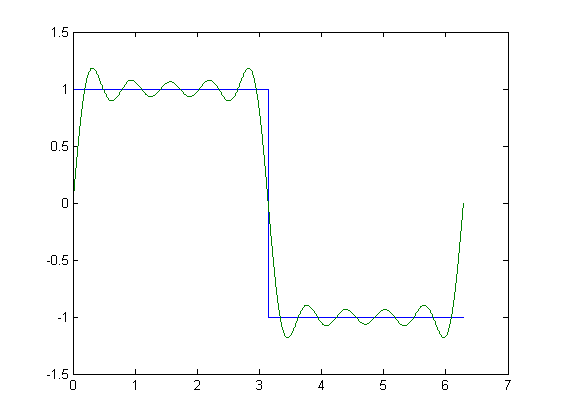
\includegraphics[width=0.7\linewidth]{HW_FourierSeries3}
\caption{Fourier series approximation of the square wave signal with 50 basis functions.}
\label{fig:HW_FourierSeries3}
\end{figure}

The Fourier series approximation of the square wave function using 50 sine coefficients is shown in Figure \ref{fig:HW_FourierSeries3}. As the approximation of the Fourier series to the square wave becomes better, the peaks at the 'shoulders' will become more and more pronounced. This effect is called the \href{http://en.wikipedia.org/wiki/Gibbs_phenomenon}{Gibbs phenomenon}, and in image processing we call this effect "ringing".\\ 

\textbf{Worked example 2}\\

Figure \ref{fig:HW_FourierSeries4} shows a saw tooth signal on the interval $[0, 2 \pi]$.

\begin{equation} \label{Eqn:HW_FourierSeries7}
\begin{split}
[0,  \pi] \implies &f(t) = t\\
[\pi,  2\pi] \implies &f(t) = t- 2 \pi
\end{split}
\end{equation}

\begin{figure}
\centering
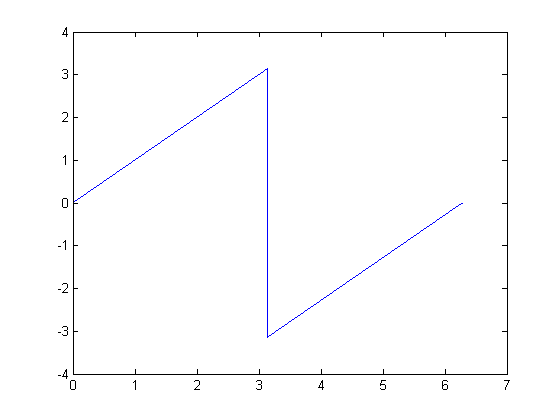
\includegraphics[width=0.7\linewidth]{HW_FourierSeries4}
\caption{Sawtooth signal on the interval $[0, 2 \pi]$.}
\label{fig:HW_FourierSeries4}
\end{figure}

It is clear from the signal that the mean value is zero, therefore $c_0$ is zero. This signal is obviously odd since $f(-t) = -f(t)$, therefore all $a_n$ are zero. Now we need to calculate the $b_n$ coefficients.

\begin{equation}\label{HW_FourierSeries8}
 b_n = \frac{1}{\pi }\int\limits_{0}^{2\pi }{f\left( t \right)\sin ntdt} = \frac{1}{\pi}\int\limits_{0}^{\pi}{t \sin nt dt} + \frac{1}{\pi }\int\limits_{\pi}^{2\pi}{(t- 2 \pi) \sin nt dt}
\end{equation}

which can be written as (watch the limits change):

\begin{equation}\label{HW_FourierSeries9}
 b_n = \frac{1}{\pi}\int\limits_{0}^{2\pi}{t \sin nt dt} - 2\int\limits_{\pi}^{2\pi}{\sin nt dt}
\end{equation}

Let's do the first term first: It is clear that we need to use partial integration $\int f'g = fg - \int fg'$, the smart choice is now: 

\begin{align}\label{Eqn:HW_FourierSeries8}
g&:t\\
g'&: 1\\
f'&: \sin nt\\
f&: \dfrac{-1}{n} \cos nt
\end{align}

Substitution gives:

\begin{equation}\label{HW_FourierSeries10}
\dfrac{1}{\pi} \int_{0}^{2 \pi} t \sin nt dt = \dfrac{1}{\pi} \left[ t \dfrac{-1}{n} \cos nt \right]_0^{2\pi} - \dfrac{1}{\pi} \int_{0}^{2 \pi} \dfrac{-1}{n} \cos nt dt
\end{equation}

Inserting the limits gives:

\begin{equation}\label{HW_FourierSeries11}
\dfrac{1}{\pi} \left[ 2 \pi \dfrac{-1}{n} \cos n 2 \pi -0  \right] - \left[ \dfrac{-1}{\pi n^2} \sin nt  \right]_0^{2\pi} = \dfrac{-2}{n} -0 = \dfrac{-2}{n}  
\end{equation}

We still have the second term as follows:

\begin{equation}\label{HW_FourierSeries12}
 - 2\int\limits_{\pi}^{2\pi}{\sin nt dt} = \left[  \dfrac{2}{n}\cos nt \right]_\pi ^{2\pi} = \dfrac{2}{n}\left[ 1 - (-1)^n \right] 
\end{equation}

The sum is now:

\begin{equation}\label{HW_FourierSeries13}
 \dfrac{-2}{n} + \dfrac{2}{n}\left[ 1 - (-1)^n \right] = \dfrac{-2}{n}(-1)^n
\end{equation}

The first four coefficients are $2 (n=1), -1 (n=2), \dfrac{2}{3} (n=3), - \dfrac{1}{2} (n=4)$, verify this in Figure \ref{fig:HW_FourierSeries5}. The Fourier series approximation of the sawtooth function using 50 basis functions is shown in Figure \ref{fig:HW_FourierSeries6}\\

\begin{figure}
\centering
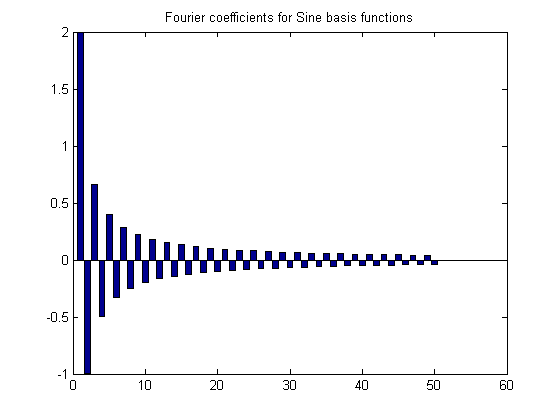
\includegraphics[width=0.7\linewidth]{HW_FourierSeries5}
\caption{Fourier coefficients of a sawtooth signal on the interval $[0, 2 \pi]$.}
\label{fig:HW_FourierSeries5}
\end{figure}

\begin{figure}
\centering
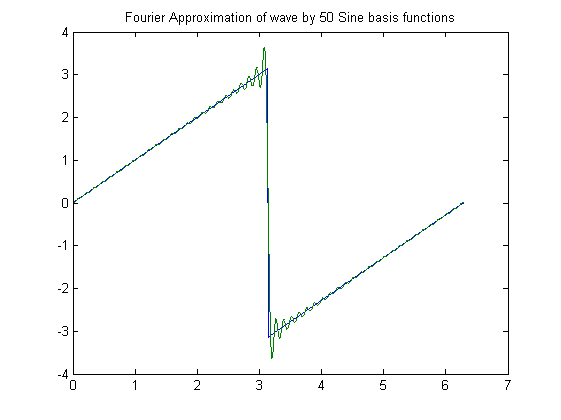
\includegraphics[width=0.7\linewidth]{HW_FourierSeries6}
\caption{Fourier series approximation of the sawtooth signal with 50 basis functions.}
\label{fig:HW_FourierSeries6}
\end{figure}

\cleardoublepage

\begin{center}
\textbf{Your homework starts here:}
\end{center}

A triangular input signal as shown in Figure \ref{fig:HW_FourierSeries7} is given on the interval $[0, 2 \pi]$. The functional form of this shape is:

\begin{equation} \label{Eqn:HW_FourierSeries14}
\begin{split}
[0,  \pi] \implies &f(t) = \dfrac{\pi}{2} -t\\
[\pi, 2 \pi ] \implies &f(t) = - \dfrac{3 \pi}{2} + t\\ 
\end{split}
\end{equation}
 
Calculate the Fourier coefficients of this function. 
\textbf{Use LaTex functionality, so just continue this document, and extend it to include your answer. Submit the pdf file of this document and don't forget to put your name at the top.} You do NOT need to show the Fourier coefficients in a graph, we'll do that in the lab.

\begin{figure}
\centering
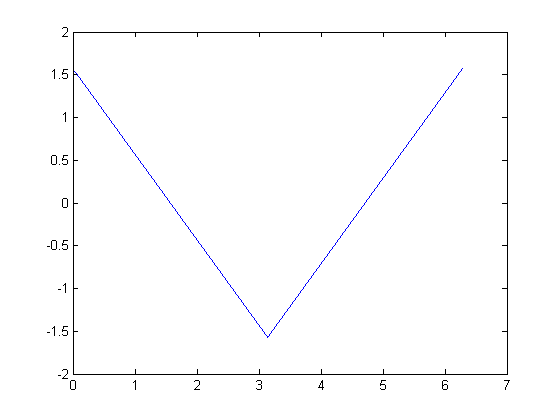
\includegraphics[width=0.7\linewidth]{HW_FourierSeries7}
\caption{Triangular signal on the interval $[0, 2 \pi]$}
\label{fig:HW_FourierSeries7}
\end{figure}

\end{document}